% =========================================================================
% MÓDULO 7: ANEXOS ADICIONALES DE DEFENSA PARA PREGUNTAS DEL JURADO (A7 A A20)
% =========================================================================

% --- ÍNDICE INTERACTIVO DE ANEXOS ADICIONALES ---
\begin{frame}{\'Indice de Anexos Adicionales para Preguntas del Jurado}{Respaldo t\'ecnico exhaustivo organizado por eje tem\'atico de defensa \cite{rodas_valencia_tpe_ecog}}
  \label{anexo:indice_extra}
  \vspace{-1.5mm}
  \begin{columns}[T,onlytextwidth]
    \begin{column}{0.49\textwidth}
      \begin{block}{1. Preprocesamiento y Filtrado Espectral}
        \tiny
        \begin{itemize}\setlength{\itemsep}{-0.5pt}
          \item \hyperlink{anexo:exclusion_canales}{\beamerbutton{Anexo A7}} Exclusi\'on fija de canales sin etiquetas (\texttt{c54, c20, c37, c49}).
          \item \hyperlink{anexo:cmr_notch}{\beamerbutton{Anexo A8}} Ecuaci\'on CMR vs.\ CAR y filtro FIR Notch ($1651$ taps).
          \item \hyperlink{anexo:ersp_antialias}{\beamerbutton{Anexo A9}} Justificaci\'on High-Gamma y decimaci\'on Antialias Kaiser.
          \item \hyperlink{anexo:ablacion_preproc}{\beamerbutton{Anexo A10}} Ablaciones secundarias de preprocesamiento (\texttt{P0, P1, P3, P5}).
        \end{itemize}
      \end{block}
      \vspace{-2.5mm}
      \begin{block}{2. Etiquetas, Auditor\'ia Antifuga y Ablaciones}
        \tiny
        \begin{itemize}\setlength{\itemsep}{-0.5pt}
          \item \hyperlink{anexo:zoh_overlap}{\beamerbutton{Anexo A11}} Desescalonado ZOH ($25\text{ Hz}$), purga $P=256$ y \textit{Overlap-Add}.
          \item \hyperlink{anexo:auditoria_v01_v14}{\beamerbutton{Anexo A12}} Huella SHA-256 y las 14 compuertas \texttt{V01--V14} (\texttt{pytest}).
          \item \hyperlink{anexo:ablaciones_detalle}{\beamerbutton{Anexo A13}} Desglose \texttt{A0}--\texttt{A5}/\texttt{A5b} y deltas apareados ($14/15$ folds).
        \end{itemize}
      \end{block}
    \end{column}

    \begin{column}{0.49\textwidth}
      \begin{block}{3. Par\'ametros, Checkpoint, TPE y Test Oficial}
        \tiny
        \begin{itemize}\setlength{\itemsep}{-0.5pt}
          \item \hyperlink{anexo:a5b_vs_a5_params}{\beamerbutton{Anexo A14}} Matem\'atica \texttt{A5b} vs.\ \texttt{A5} y conteo de par\'ametros ($9.35\text{--}28.03\text{ M}$).
          \item \hyperlink{anexo:checkpoint_retrospectivo}{\beamerbutton{Anexo A15}} Simulaci\'on retrospectiva de checkpoint ($0.6837 \to 0.7330$).
          \item \hyperlink{anexo:tpe_diagnostico}{\beamerbutton{Anexo A16}} Matem\'atica TPE ($\ell/g$), descomposici\'on de $+0.0672$ y 60 folds.
          \item \hyperlink{anexo:protocolos_test_brecha}{\beamerbutton{Anexo A17}} Protocolos de Test ($0.6333$ vs.\ $0.6669$) y brecha CV vs.\ Test.
        \end{itemize}
      \end{block}
      \vspace{-2.5mm}
      \begin{block}{4. Estado del Arte, Trazabilidad CSV y Poda}
        \tiny
        \begin{itemize}\setlength{\itemsep}{-0.5pt}
          \item \hyperlink{anexo:comparacion_dtcnet_dedos}{\beamerbutton{Anexo A18}} Comparaci\'on celda a celda ($15$ pares) \texttt{A5} vs.\ \textit{DTCNet} (2025).
          \item \hyperlink{anexo:trazabilidad_csv}{\beamerbutton{Anexo A19}} Matriz completa de 16 archivos CSV y 6 reglas de c\'alculo.
          \item \hyperlink{anexo:poda_y_privacidad}{\beamerbutton{Anexo A20}} Gobernanza de datos cl\'inicos y formulaci\'on de Poda Estructurada.
        \end{itemize}
      \end{block}
    \end{column}
  \end{columns}
\end{frame}

% --- ANEXO A7: EXCLUSIÓN FIJA DE CANALES DEFECTUOSOS ---
\begin{frame}{Anexo A7: Auditor\'ia de Calidad y Exclusi\'on Fija de Canales Defectuosos}{Pregunta del jurado: ?`Por qu\'e se excluyeron electrodos espec\'ificos y c\'omo garantizan que no usaron las etiquetas para elegirlos?}
  \label{anexo:exclusion_canales}
  \begin{columns}[T,onlytextwidth]
    \begin{column}{0.32\textwidth}
      \centering
      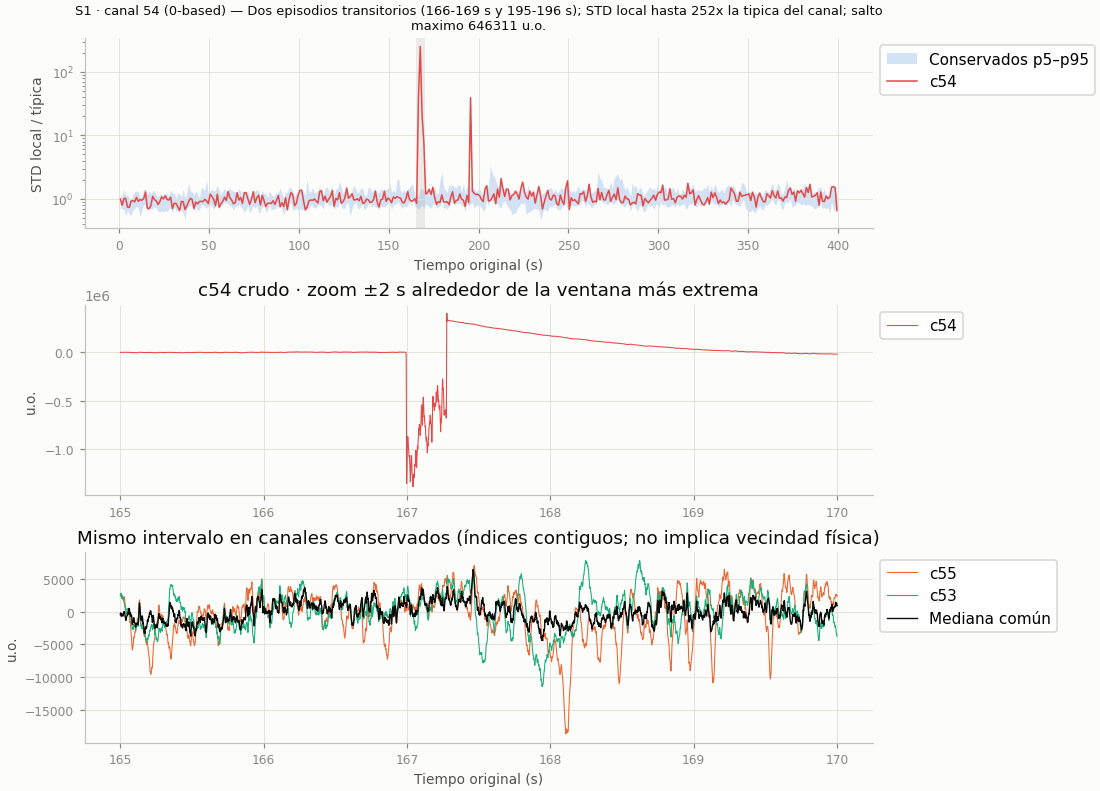
\includegraphics[width=\linewidth,height=0.36\textheight,keepaspectratio]{imgs/s02_S1_c054.png}
      \figcap{A.6}{Anomal\'ia en \texttt{S1-c054} ($62 \to 61$). \textbf{Fuente:} Obtenida de GitHub \cite{rodas_valencia_tpe_ecog}.}
    \end{column}
    \begin{column}{0.32\textwidth}
      \centering
      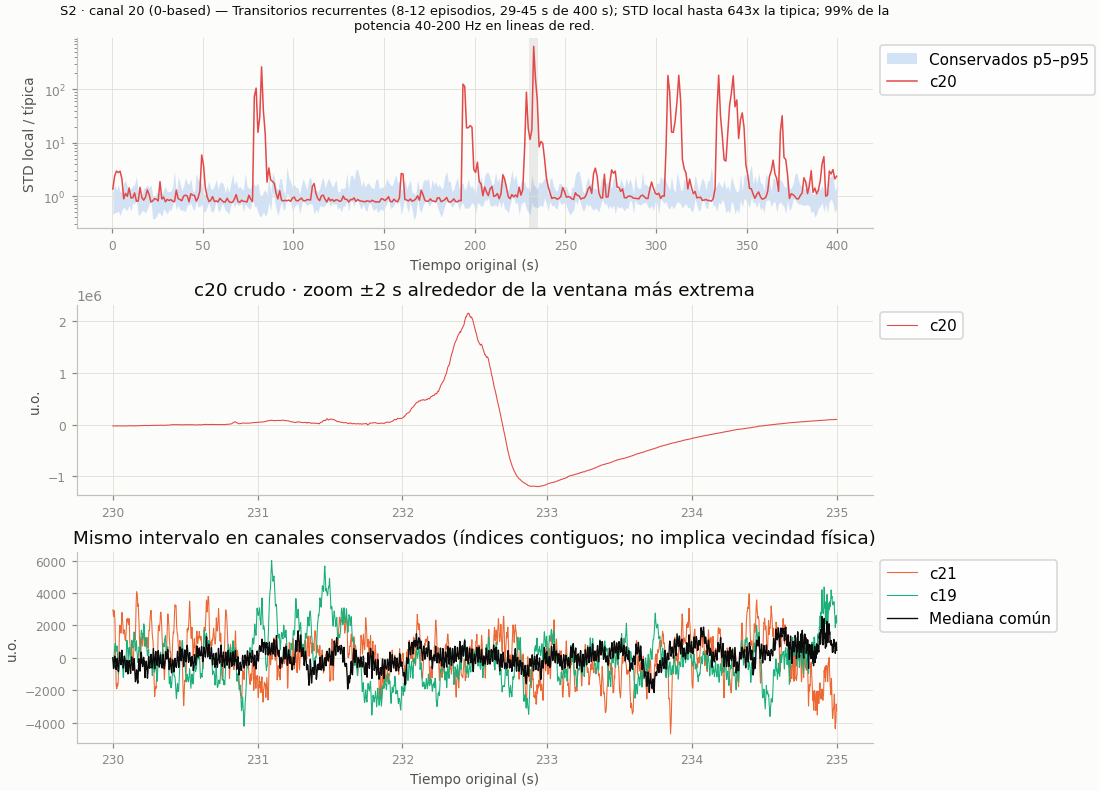
\includegraphics[width=\linewidth,height=0.36\textheight,keepaspectratio]{imgs/s02_S2_c020.png}
      \figcap{A.7}{Artefactos en \texttt{S2-c020} ($48 \to 46$). \textbf{Fuente:} Obtenida de GitHub \cite{rodas_valencia_tpe_ecog}.}
    \end{column}
    \begin{column}{0.32\textwidth}
      \centering
      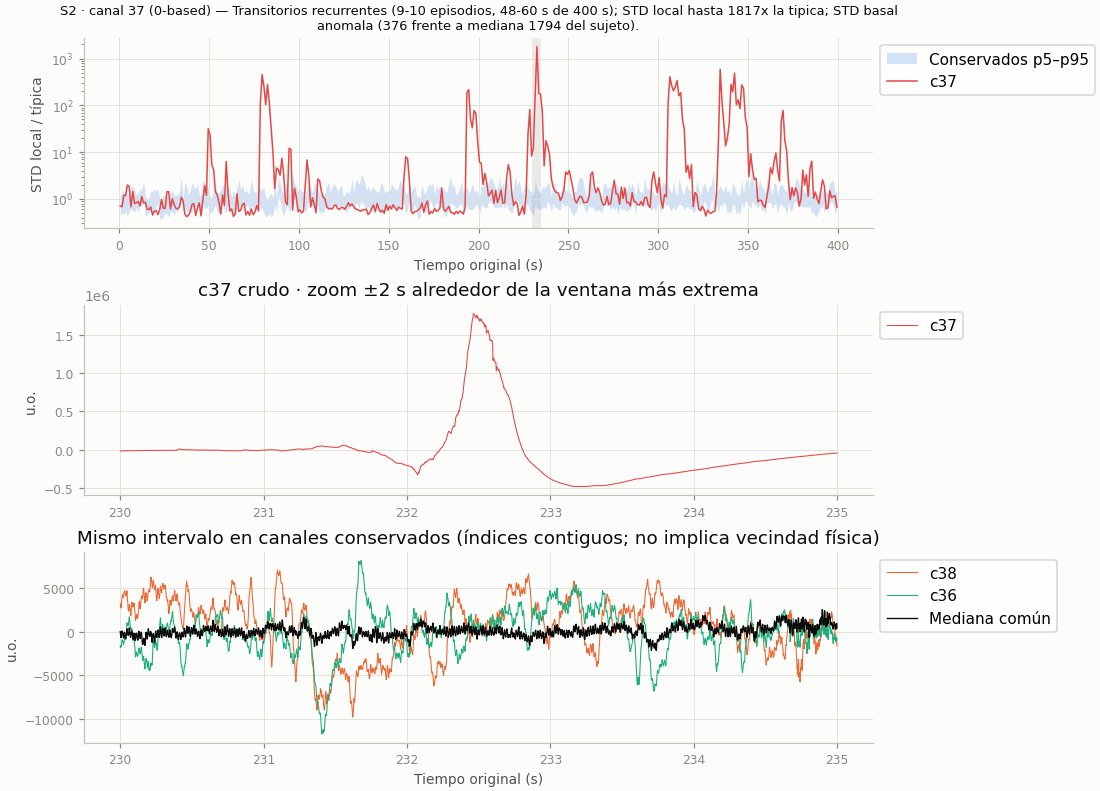
\includegraphics[width=\linewidth,height=0.36\textheight,keepaspectratio]{imgs/s02_S2_c037.png}
      \figcap{A.8}{Transitorio en \texttt{S2-c037} ($>1800\sigma$). \textbf{Fuente:} Obtenida de GitHub \cite{rodas_valencia_tpe_ecog}.}
    \end{column}
  \end{columns}

  \vspace{1mm}
  \begin{block}{Inspecci\'on Ciega a Etiquetas y Extirpaci\'on Previa a la Referencia Espacial}
    \scriptsize
    \begin{itemize}\setlength{\itemsep}{1.5pt}
      \item \textbf{Auditor\'ia exclusivamente sobre ECoG crudo de desarrollo:} La detecci\'on de saturaci\'on y varianza an\'omala se ejecut\'o sin consultar las trayectorias del guante (\texttt{dataglove}), bloqueando cualquier sesgo de selecci\'on de caracter\'isticas \cite{rodas_valencia_tpe_ecog}.
      \item \textbf{Canales extirpados antes de la CMR:} \texttt{S1}: canal $54$ ($62 \to 61$); \texttt{S2}: canales $20$ y $37$ ($48 \to 46$); \texttt{S3}: canal $49$ ($64 \to 63$). \hfill\hyperlink{anexo:indice_extra}{\beamerbutton{Volver al \'Indice Extra}}
    \end{itemize}
  \end{block}
\end{frame}

% --- ANEXO A8: CMR VS CAR Y FILTRADO FIR NOTCH ---
\begin{frame}{Anexo A8: Referencia Com\'un a la Mediana (CMR) vs.\ CAR y Filtrado FIR Notch}{Pregunta del jurado: ?`Por qu\'e usar CMR en lugar del promedio com\'un (CAR) y c\'omo se elimin\'o el ruido de l\'inea de $60\text{ Hz}$?}
  \label{anexo:cmr_notch}
  \begin{columns}[T,onlytextwidth]
    \begin{column}{0.48\textwidth}
      \centering
      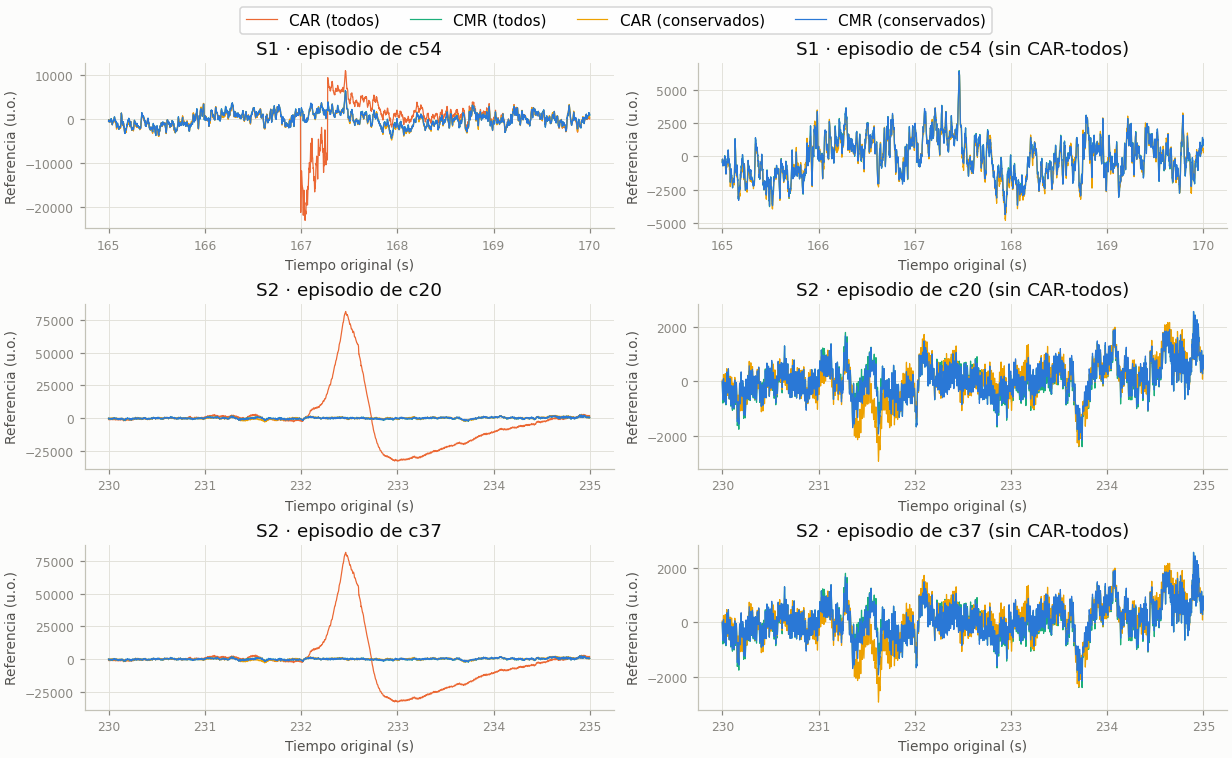
\includegraphics[width=\linewidth,height=0.37\textheight,keepaspectratio]{imgs/s03_reference_episodes.png}
      \figcap{A.9}{Inmunidad de CMR frente a contaminaci\'on global en CAR. \textbf{Fuente:} Obtenida de GitHub \cite{rodas_valencia_tpe_ecog}.}
    \end{column}
    \begin{column}{0.48\textwidth}
      \centering
      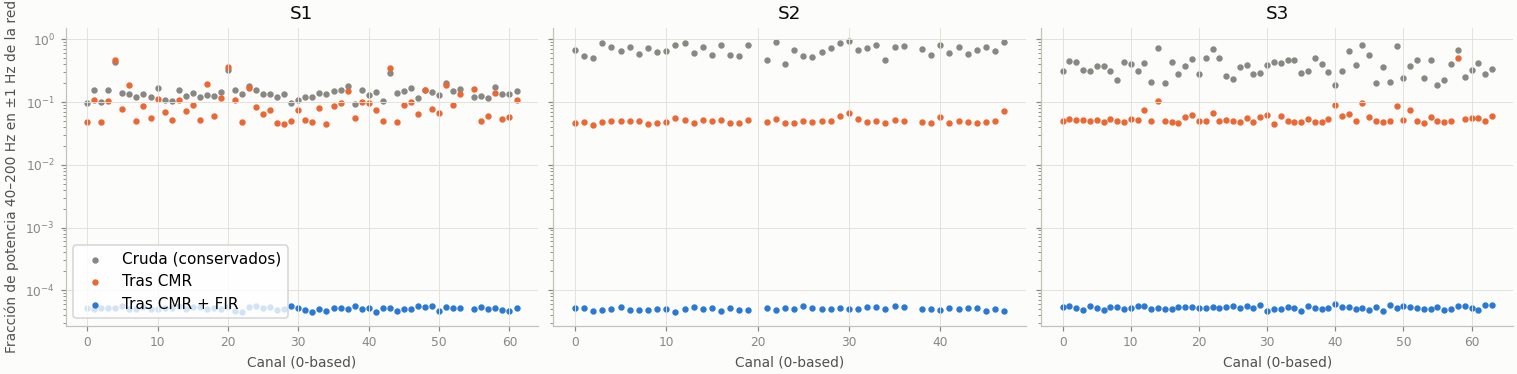
\includegraphics[width=\linewidth,height=0.37\textheight,keepaspectratio]{imgs/s05_line_fraction.png}
      \figcap{A.10}{Supresi\'on el\'ectrica en $60, 120, 180\text{ Hz}$ con Notch triple. \textbf{Fuente:} Obtenida de GitHub \cite{rodas_valencia_tpe_ecog}.}
    \end{column}
  \end{columns}

  \vspace{0.5mm}
  \begin{block}{Fundamento Matem\'atico de Robustez Espacial y Espectral}
    \scriptsize
    \begin{itemize}\setlength{\itemsep}{1.5pt}
      \item \textbf{Referencia Com\'un a la Mediana (CMR):} $\widetilde{X}_{c,t} = X_{c,t} - \operatorname{mediana}_{j \in C_{\text{v\'alidos}}}(X_{j,t})$. La mediana posee un \textbf{punto de ruptura del $50\%$} e impide que un artefacto local residual contamine a los canales sanos, a diferencia del promedio CAR \cite{Schalk2011,rodas_valencia_tpe_ecog}.
      \item \textbf{Filtro FIR Notch de fase cero ($1651$ taps):} Aten\'ua $>40\text{ dB}$ en $\mathbf{60, 120\text{ y }180\text{ Hz}}$ sin distorsi\'on de fase. \hfill\hyperlink{anexo:indice_extra}{\beamerbutton{Volver al \'Indice Extra}}
    \end{itemize}
  \end{block}
\end{frame}

% --- ANEXO A9: JUSTIFICACIÓN HIGH-GAMMA Y DECIMACIÓN ANTIALIAS KAISER ---
\begin{frame}{Anexo A9: Justificaci\'on High-Gamma ($40\text{--}200\text{ Hz}$) y Decimaci\'on Antialias Kaiser}{Pregunta del jurado: ?`Por qu\'e acotar las wavelets de Morlet a $40\text{--}200\text{ Hz}$ y c\'omo evitaron el aliasing al bajar de $1000\text{ Hz}$ a $100\text{ Hz}$?}
  \label{anexo:ersp_antialias}
  \begin{columns}[T,onlytextwidth]
    \begin{column}{0.48\textwidth}
      \centering
      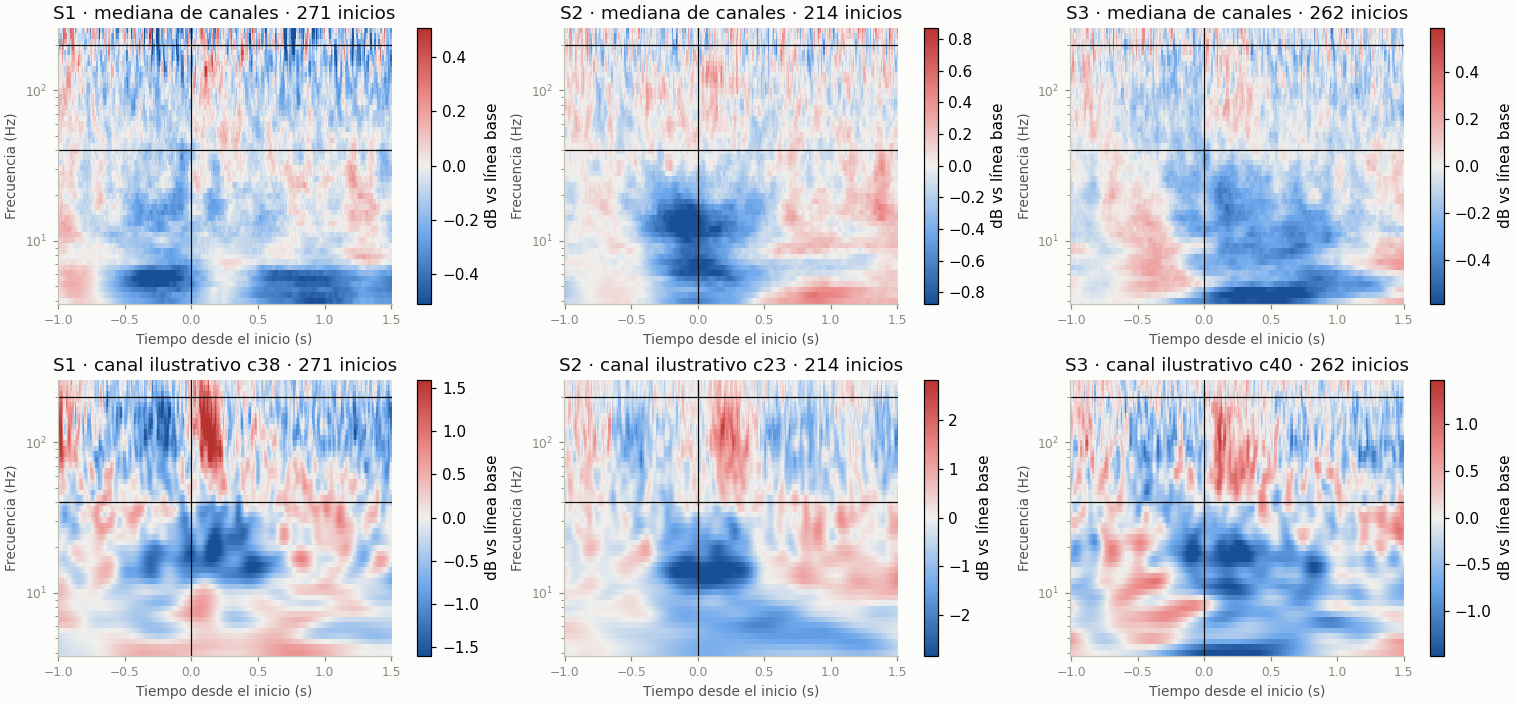
\includegraphics[width=\linewidth,height=0.37\textheight,keepaspectratio]{imgs/s04_ersp.png}
      \figcap{A.11}{Actividad motora acoplada en banda High-Gamma ($40\text{--}200\text{ Hz}$). \textbf{Fuente:} Obtenida de GitHub \cite{rodas_valencia_tpe_ecog}.}
    \end{column}
    \begin{column}{0.48\textwidth}
      \centering
      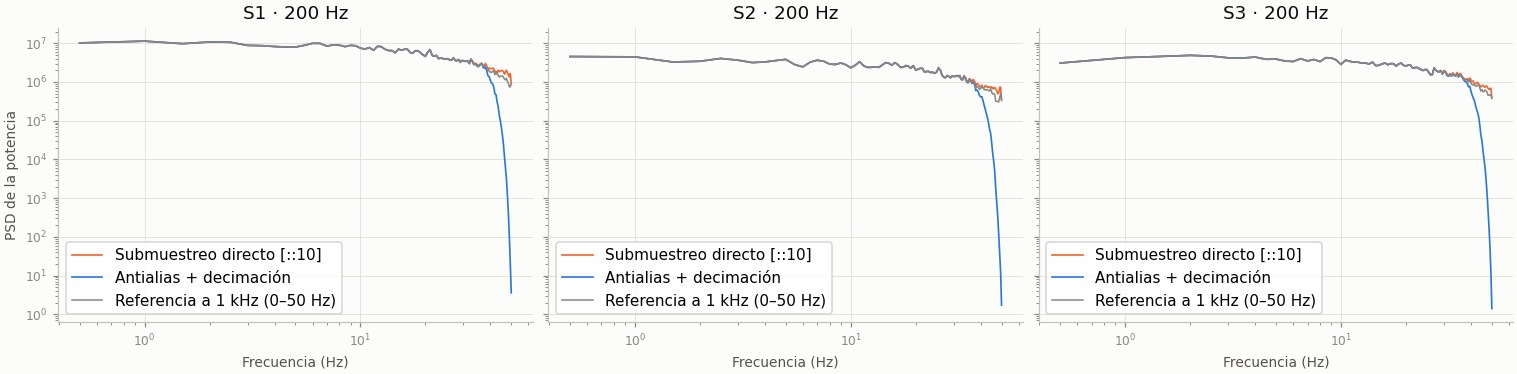
\includegraphics[width=\linewidth,height=0.37\textheight,keepaspectratio]{imgs/s07_naive_vs_antialias.png}
      \figcap{A.12}{Decimaci\'on FIR Kaiser ($243$ taps, $-60\text{ dB}$). \textbf{Fuente:} Obtenida de GitHub \cite{rodas_valencia_tpe_ecog}.}
    \end{column}
  \end{columns}

  \vspace{0.5mm}
  \begin{block}{Acoplamiento Tiempo-Frecuencia y Prevenci\'on del Plegado Espectral (\textit{Aliasing})}
    \scriptsize
    \begin{itemize}\setlength{\itemsep}{1.5pt}
      \item \textbf{Banco CWT de Morlet ($40$ escalas logar\'itmicas, $n_c=7$ ciclos):} Captura la envolvente de potencia sin\'aptica local en $40\text{--}200\text{ Hz}$ \cite{kaplan2019decoding,Bundy2016}.
      \item \textbf{Decimaci\'on Antialias ($1000\text{ Hz} \to 100\text{ Hz}$, Nyquist $=50\text{ Hz}$):} El filtro FIR con ventana de Kaiser ($243$ taps, rechazo de $-60\text{ dB}$) elimina fluctuaciones r\'apidas antes de diezmar por factor $10$, evitando el plegado espectral sobre la envolvente \cite{rodas_valencia_tpe_ecog}. \hfill\hyperlink{anexo:indice_extra}{\beamerbutton{Volver al \'Indice Extra}}
    \end{itemize}
  \end{block}
\end{frame}

% --- ANEXO A10: ABLACIONES SECUNDARIAS DE PREPROCESAMIENTO ---
\begin{frame}{Anexo A10: Ablaciones Secundarias de Preprocesamiento (\texttt{P0}, \texttt{P1}, \texttt{P3}, \texttt{P5})}{Pregunta del jurado: ?`Qu\'e ocurri\'o cuando probaron variantes del preprocesamiento sobre la red base \texttt{A0}?}
  \label{anexo:ablacion_preproc}
  \centering
  \resizebox{\textwidth}{!}{%
    \renewcommand{\arraystretch}{1.18}
    \begin{tabular}{>{\bfseries}l l c c c c c}
      \toprule
      \rowcolor{ipnDark}
      \textcolor{white}{Variante} & \textcolor{white}{Descripci\'on del cambio en el pipeline (sobre red base \texttt{A0}, \'epoca 50)} & \textcolor{white}{\texttt{S1}} & \textcolor{white}{\texttt{S2}} & \textcolor{white}{\texttt{S3}} & \textcolor{white}{Media CV ($r$)} & \textcolor{white}{$\Delta r$ vs.\ \texttt{P0}} \\
      \midrule
      \texttt{P0} (Fijado) & Pipeline de referencia fijado (Exclusi\'on + CMR + FIR + 40 Morlet + Kaiser) & $0.4990$ & $0.4289$ & $0.7187$ & $0.5489$ & --- \\
      \rowcolor{rowHighlight}
      \texttt{P1} & Sin referencia espacial CMR (conservando el resto de \texttt{P0} id\'entico) & $0.4992$ & $\mathbf{0.5446}$ & $0.7220$ & $\mathbf{0.5886}$ & $\mathbf{+0.0397}$ \\
      \texttt{P3} & Variante espectral secundaria evaluada en Secci\'on 3.6 & --- & --- & --- & $0.5572$ & $+0.0084$ \\
      \rowcolor{rowLight}
      \texttt{P5} & Variante de acondicionamiento secundaria evaluada en Secci\'on 3.6 & --- & --- & --- & $0.5498$ & $+0.0009$ \\
      \bottomrule
    \end{tabular}%
  }
  \fuente{Creaci\'on propia, obtenida del repositorio GitHub \cite{rodas_valencia_tpe_ecog}.}

  \vspace{1.5mm}
  \begin{block}{Lectura Metodol\'ogica Rigurosa (Secci\'on 3.6 del Reporte Experimental)}
    \scriptsize
    \begin{itemize}\setlength{\itemsep}{2.5pt}
      \item \textbf{Origen de la diferencia en \texttt{P1}:} Al evaluar \texttt{P1} (sin CMR) sobre la arquitectura inicial \texttt{A0} en la \'epoca 50, la media subi\'o a $\mathbf{0.5886}$ ($\Delta = +0.0397$), concentrada casi por completo en el \textbf{Sujeto 2 ($\mathbf{+0.1157}$)}.
      \item \textbf{Por qu\'e \texttt{P0} se mantuvo fijo:} La b\'usqueda bayesiana \textbf{TPE} y las ablaciones \texttt{A1}--\texttt{A5} se ejecutaron con \texttt{P0} congelado para garantizar comparabilidad estricta; \texttt{P1} no fue evaluado de forma controlada con la arquitectura final \texttt{A5} optimizada.
      \item \textbf{Interpretaci\'on honesta:} Por ello, \texttt{P0} se documenta como el \textbf{pipeline de referencia fijado para la comparabilidad experimental}, y no como el mejor preprocesamiento posible demostrado \cite{rodas_valencia_tpe_ecog}. \hfill\hyperlink{anexo:indice_extra}{\beamerbutton{Volver al \'Indice Extra}}
    \end{itemize}
  \end{block}
\end{frame}

% --- ANEXO A11: DESESCALONADO ZOH, PURGA Y OVERLAP-ADD ---
\begin{frame}{Anexo A11: Desescalonado ZOH ($25\text{ Hz}$), Purga ($P=256$) y \textit{Overlap-Add}}{Pregunta del jurado: ?`C\'omo se corrigi\'o el escalonado del guante y c\'omo se reconstruye la trayectoria continua para medir Pearson?}
  \label{anexo:zoh_overlap}
  \begin{columns}[c,onlytextwidth]
    \begin{column}{0.48\textwidth}
      \begin{block}{1. Desescalonado ZOH y Purga Antifuga}
        \scriptsize
        \begin{itemize}\setlength{\itemsep}{2pt}
          \item \textbf{Almacenamiento ZOH:} El guante muestrea a $25\text{ Hz}$ pero se repite cada $40$ muestras a $1000\text{ Hz}$: $\texttt{train\_dg}[n] = g_{\text{real}}[\lfloor n/40 \rfloor]$.
          \item \textbf{Spline + Adelanto:} Se extraen las muestras reales ($n=40m$), se interpola con Spline C\'ubico \textit{Not-a-Knot} a $100\text{ Hz}$ y se adelanta $\tau = 20\text{ ms}$ ($+2$ muestras).
          \item \textbf{Bordes y Purga:} Recorte de $\pm 125$ muestras por bloque ($N=7750$ v\'alidas) y purga de $\mathbf{P=256\text{ muestras}}$ en fronteras de train adyacentes a validaci\'on.
        \end{itemize}
      \end{block}

      \begin{block}{2. Reconstrucci\'on \textit{Overlap-Add} ($119$ Ventanas)}
        \scriptsize
        Se deslizan $118$ ventanas ($W=256, s=64$) m\'as la ventana $\#119$ anclada en $[7494, 7750)$, promediando $\widehat{Y}_d[k] = S_d[k]/C[k]$ antes de medir Pearson sobre la trayectoria completa.
      \end{block}
    \end{column}

    \begin{column}{0.49\textwidth}
      \centering
      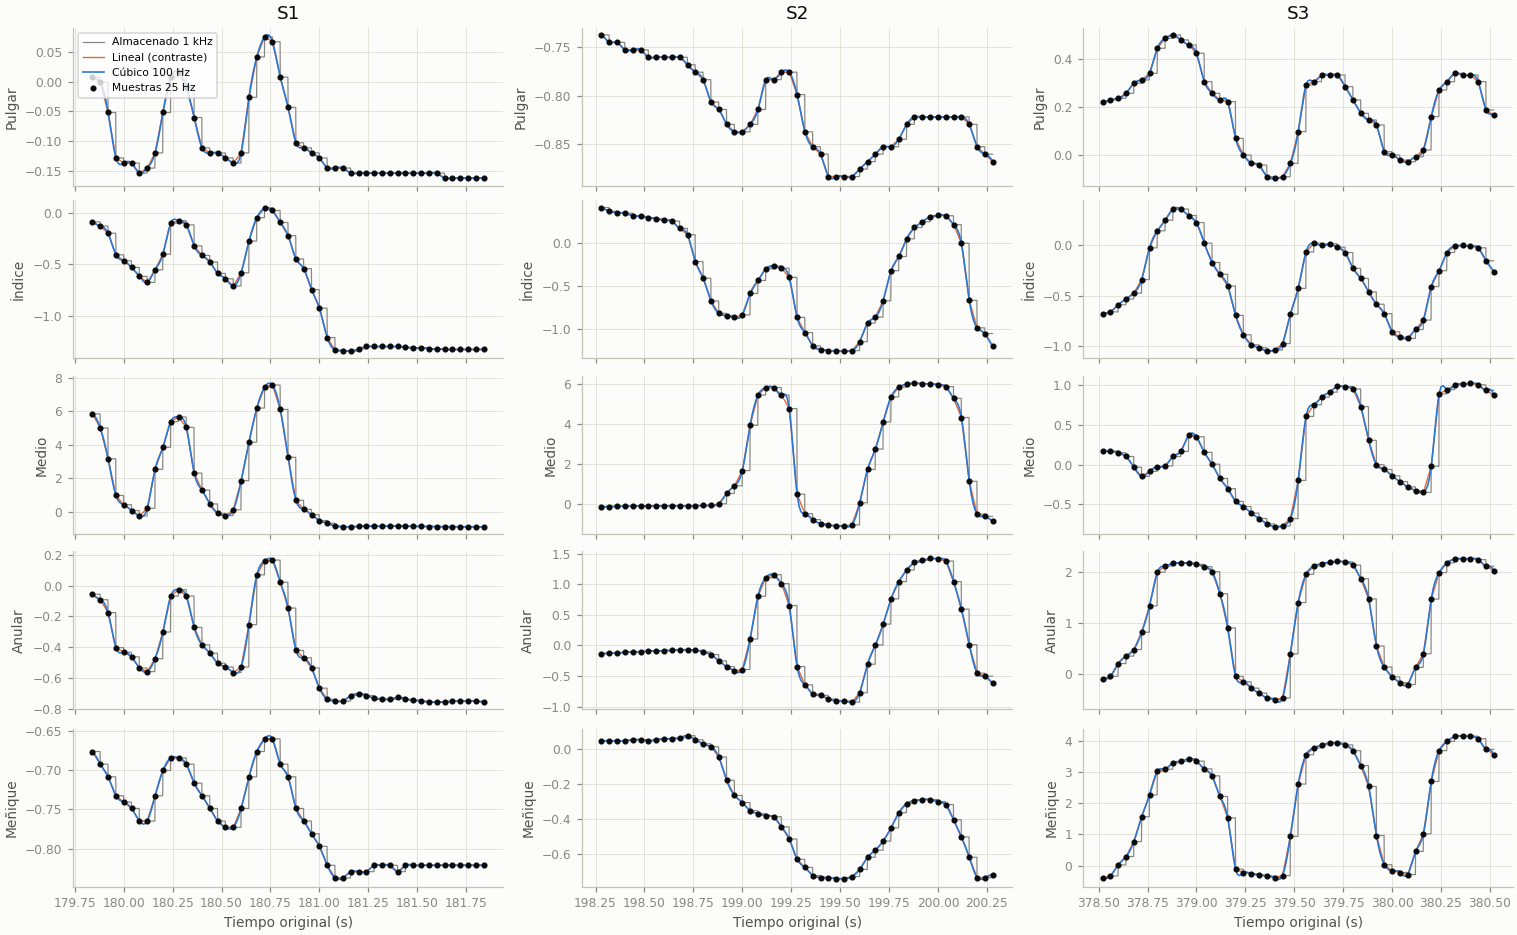
\includegraphics[width=\linewidth,height=0.45\textheight,keepaspectratio]{imgs/s08_glove_interpolation.png}
      \figcap{A.13}{Eliminaci\'on de escalones ZOH ($25\text{ Hz}$) mediante Spline C\'ubico a $100\text{ Hz}$. \textbf{Fuente:} Obtenida del repositorio GitHub \cite{rodas_valencia_tpe_ecog}.}
      \vspace{1mm}
      \hfill\hyperlink{anexo:indice_extra}{\beamerbutton{Volver al \'Indice Extra}}
    \end{column}
  \end{columns}
\end{frame}

% --- ANEXO A12: HUELLA SHA-256 Y COMPUERTAS V01-V14 ---
\begin{frame}{Anexo A12: Huella Criptogr\'afica SHA-256 y las 14 Compuertas (\texttt{V01--V14})}{Pregunta del jurado: ?`Qu\'e pruebas de software certifican que no existi\'o fuga de datos (\textit{data leakage}) entre bloques?}
  \label{anexo:auditoria_v01_v14}
  \centering
  \scriptsize
  \renewcommand{\arraystretch}{1.18}
  \begin{tabularx}{\textwidth}{>{\bfseries\color{ipnDark}}l l >{\raggedright\arraybackslash}X}
    \toprule
    \rowcolor{ipnDark}
    \textcolor{white}{Bloque} & \textcolor{white}{Compuertas \texttt{pytest}} & \textcolor{white}{Verificaci\'on automatizada y garant\'ia metodol\'ogica certificada} \\
    \midrule
    \texttt{V01--V03} & Integridad de origen y canales & Inmutabilidad de archivos \texttt{.mat} crudos, bloqueo estricto de \texttt{test\_labels} durante desarrollo y exclusi\'on fija de canales corruptos previa al c\'alculo de la mediana espacial CMR. \\
    \rowcolor{rowLight}
    \texttt{V04--V06} & Partici\'on, escalado y latencia & Separaci\'on cronol\'ogica con purga $P=256$, ajuste de \texttt{RobustScaler}$(10,90)$ y \texttt{MinMaxScaler}$[0,1]$ exclusivamente sobre train, y alineaci\'on temporal $\tau=20\text{ ms}$. \\
    \rowcolor{rowHighlight}
    \texttt{V07--V08} & \textbf{Experimento contrafactual bit a bit} & Se inyecta un impulso gigante ($\mathbf{10^6 \times \max|\text{ECoG}|}$) en el bloque de validaci\'on crudo; al regenerar el fold, los tensores v\'alidos de entrenamiento permanecen \textbf{id\'enticos bit a bit ($\text{tolerancia} = 0.0$)}. \\
    \texttt{V09--V14} & Soporte DSP, OLA y m\'etricas & Verificaci\'on de bordes FIR/Morlet ($\pm 125$ muestras), conteo exacto de $119$ ventanas, cobertura $C[k]\ge 1$ en \textit{overlap-add}, validez de \texttt{A0--A5} y f\'ormulas de $r$, $\operatorname{CCC}$ y $\operatorname{MSE}$. \\
    \bottomrule
  \end{tabularx}
  \fuente{Creaci\'on propia, obtenida del repositorio GitHub \cite{rodas_valencia_tpe_ecog}.}

  \vspace{2mm}
  \begin{block}{Identificador Inmutable \texttt{pipeline\_id} (SHA-256)}
    \scriptsize
    Cada artefacto preprocesado registra un hash criptogr\'afico \textbf{SHA-256} derivado de los hiperpar\'ametros de filtrado, escalado y partici\'on, impidiendo mezclar tensores de distintas configuraciones \cite{rodas_valencia_tpe_ecog}. \hfill\hyperlink{anexo:indice_extra}{\beamerbutton{Volver al \'Indice Extra}}
  \end{block}
\end{frame}

% --- ANEXO A13: DESGLOSE COMPLETO DE ABLACIONES ARQUITECTÓNICAS ---
\begin{frame}{Anexo A13: Desglose de Ablaciones Arquitect\'onicas (\texttt{A0}--\texttt{A5}, \texttt{A5b}) y Deltas}{Pregunta del jurado: ?`Por qu\'e no se puede afirmar que \texttt{ConvTranspose1d} mejora el rendimiento por s\'i sola?}
  \label{anexo:ablaciones_detalle}
  \begin{columns}[c,onlytextwidth]
    \begin{column}{0.48\textwidth}
      \centering
      \resizebox{\linewidth}{!}{%
        \renewcommand{\arraystretch}{1.16}
        \begin{tabular}{>{\bfseries}l l c c}
          \toprule
          \rowcolor{ipnDark}
          \textcolor{white}{Red} & \textcolor{white}{Configuraci\'on (\'epoca 50 fija)} & \textcolor{white}{Media CV} & \textcolor{white}{$\Delta r$ vs.\ \texttt{A0}} \\
          \midrule
          \texttt{A0/P0} & Base U-Net 1D (\texttt{BatchNorm1d}) & $0.5489$ & --- \\
          \rowcolor{rowLight}
          \texttt{A1} & + \texttt{LayerNorm} por grupo temporal & $0.6094$ & $+0.0605$ \\
          \texttt{A2} & + \texttt{Dropout} espacial $p=0.10$ & $0.6219$ & $+0.0731$ \\
          \rowcolor{ipnSoft}
          \texttt{A3} & + \texttt{ConvTranspose1d} aislada & $\mathbf{0.5173}$ & $\mathbf{-0.0316}$ \\
          \texttt{A4} & + \textit{Skip} previo a \texttt{Conv1d} & $0.5806$ & $+0.0317$ \\
          \rowcolor{rowLight}
          \texttt{A5b} & Combinada (\texttt{A1+A2+A4}) con interp. & $0.6779$ & $+0.1291$ \\
          \rowcolor{rowHighlight}
          \texttt{A5} & Combinada + \texttt{ConvTranspose} \textit{depthwise} & $\mathbf{0.6837}$ & $\mathbf{+0.1349}$ \\
          \bottomrule
        \end{tabular}%
      }
      \fuente{Creaci\'on propia, obtenida del repositorio GitHub \cite{rodas_valencia_tpe_ecog}.}

      \vspace{1.5mm}
      \begin{block}{Deltas Apareados $\texttt{A0} \to \texttt{A5}$ ($14/15$ Folds $+$) }
        \tiny
        \texttt{S1}: $+0.1048$ ($4/5$ folds; \'unica excepci\'on \texttt{S1-B3} con $-0.0359$).\\
        \texttt{S2}: $\mathbf{+0.1927}$ ($5/5$ folds) \,|\, \texttt{S3}: $\mathbf{+0.1070}$ ($5/5$ folds).
      \end{block}
    \end{column}

    \begin{column}{0.49\textwidth}
      \centering
      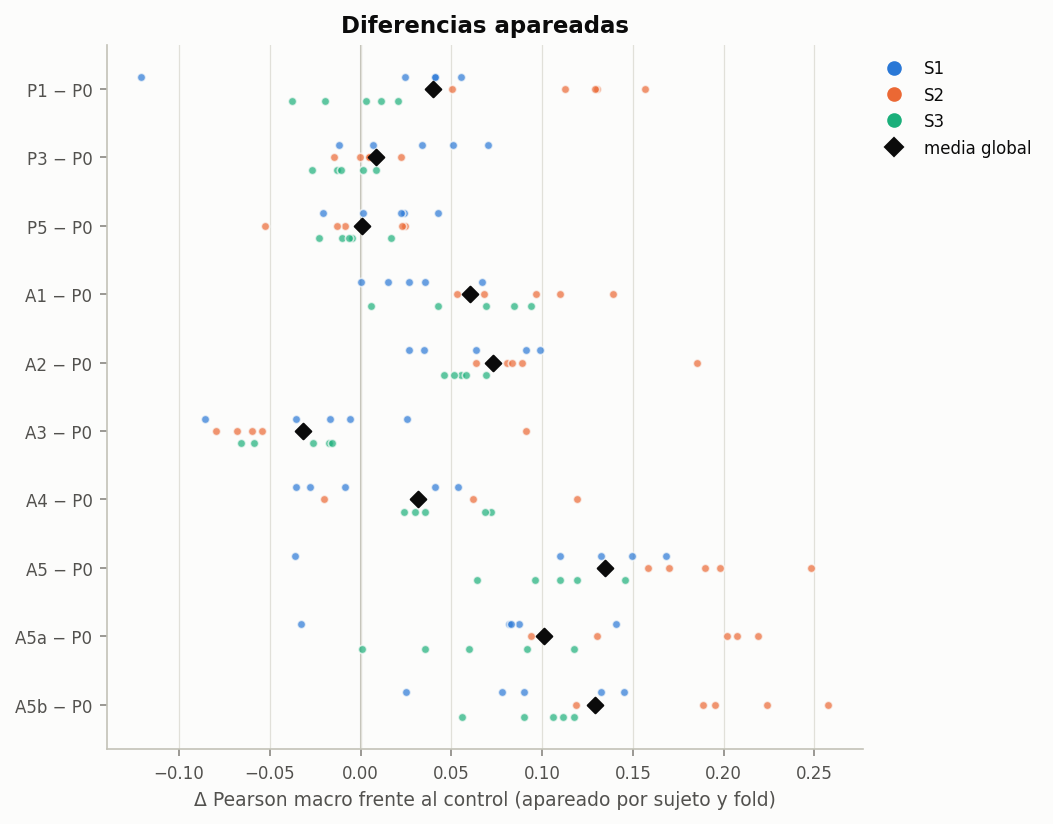
\includegraphics[width=0.48\linewidth,height=0.36\textheight,keepaspectratio]{imgs/paired_deltas.png}\hfill
      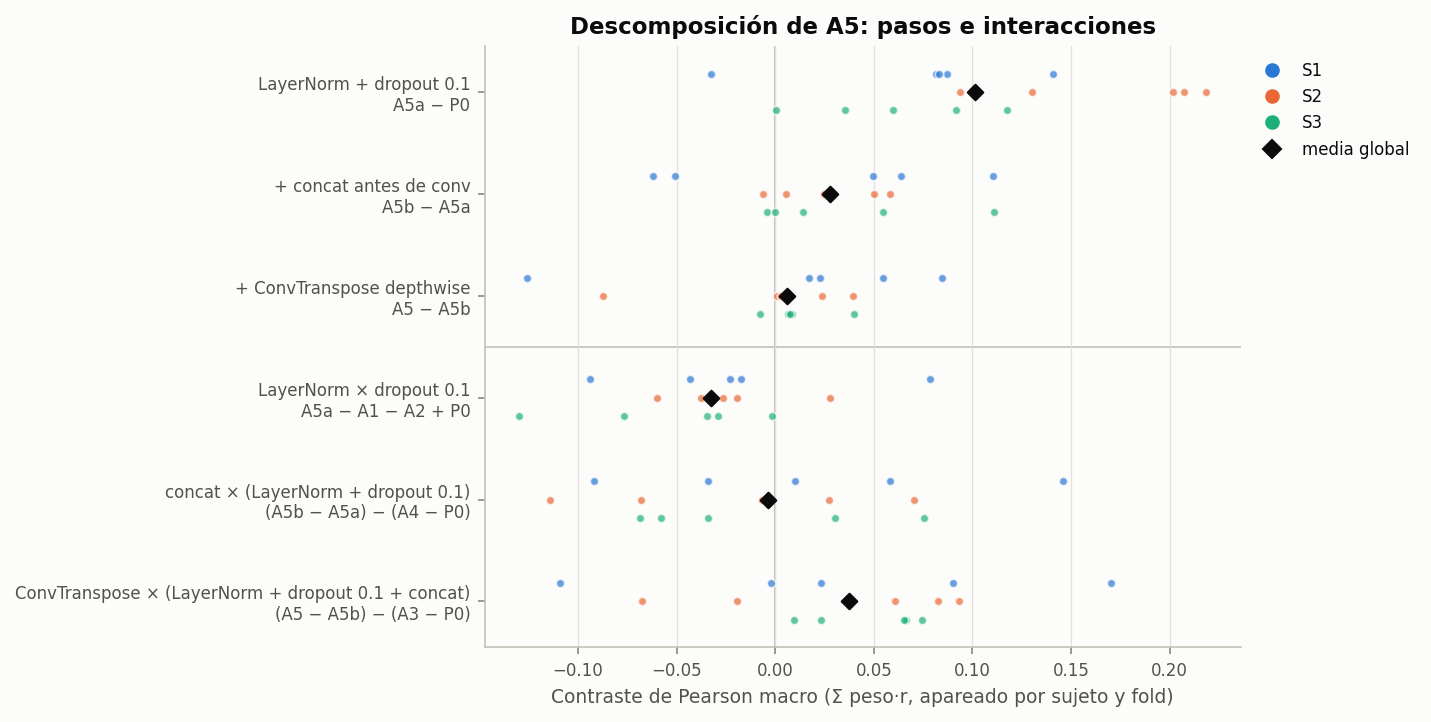
\includegraphics[width=0.48\linewidth,height=0.36\textheight,keepaspectratio]{imgs/contrasts.png}
      \figcap{A.14}{Izquierda: deltas apareados por pliegue ($\texttt{A0}\to\texttt{A5}$). Derecha: contrastes de efectos individuales y sin\'ergicos. \textbf{Fuente:} Obtenida del repositorio GitHub \cite{rodas_valencia_tpe_ecog}.}
      \vspace{1mm}
      \hfill\hyperlink{anexo:indice_extra}{\beamerbutton{Volver al \'Indice Extra}}
    \end{column}
  \end{columns}
\end{frame}

% --- ANEXO A14: MATEMÁTICA A5B VS A5 Y CONTEO DE PARÁMETROS ---
\begin{frame}{Anexo A14: Matem\'atica \texttt{A5b} vs.\ \texttt{A5} y Conteo de Par\'ametros por Sujeto}{Pregunta del jurado: ?`Cu\'al es la diferencia matem\'atica entre el decoder de \texttt{A5b} y \texttt{A5}, y cu\'antos par\'ametros tiene cada red?}
  \label{anexo:a5b_vs_a5_params}
  \begin{columns}[T,onlytextwidth]
    \begin{column}{0.48\textwidth}
      \begin{block}{1. Interpolaci\'on (\texttt{A5b}) vs.\ \texttt{ConvTranspose1d} (\texttt{A5})}
        \scriptsize
        \begin{itemize}\setlength{\itemsep}{3pt}
          \item \textbf{Variante \texttt{A5b} ($0$ par\'ametros en sobremuestreo):} Emplea interpolaci\'on lineal vectorizada con pesos geom\'etricos fijos ($0.75$ y $0.25$) para duplicar la resoluci\'on temporal en cada nivel del decodificador.
          \item \textbf{Variante \texttt{A5} (\texttt{ConvTranspose1d} \textit{depthwise}):} Configura $k=4, s=2, p=1, \text{groups}=C$, a\~nadiendo solo $\mathbf{4C\text{ pesos por nivel}}$. Incluye a la interpolaci\'on lineal como caso particular exacto y aprende el perfil de reconstrucci\'on temporal por canal \cite{rodas_valencia_tpe_ecog}.
        \end{itemize}
      \end{block}
    \end{column}

    \begin{column}{0.49\textwidth}
      \begin{block}{2. Conteo de Par\'ametros Ganadores (\texttt{tpe\_trials.csv})}
        \centering
        \resizebox{\linewidth}{!}{%
          \renewcommand{\arraystretch}{1.18}
          \begin{tabular}{>{\bfseries}l c c c r}
            \toprule
            \rowcolor{ipnDark}
            \textcolor{white}{Sujeto} & \textcolor{white}{Trial} & \textcolor{white}{Topolog\'ia ($k, L, f$)} & \textcolor{white}{Canales ECoG} & \textcolor{white}{Par\'ametros} \\
            \midrule
            \texttt{S1} & $\#10$ & $k=5, L=5, f=64$ & $61 \times 40$ & $\mathbf{9.35\text{ M}}$ \\
            \rowcolor{rowHighlight}
            \texttt{S2} & $\#30$ & $k=7, L=5, f=96$ & $46 \times 40$ & $\mathbf{28.03\text{ M}}$ \\
            \texttt{S3} & $\#26$ & $k=7, L=5, f=64$ & $63 \times 40$ & $\mathbf{12.71\text{ M}}$ \\
            \bottomrule
          \end{tabular}%
        }
        \fuente{Creaci\'on propia, obtenida del repositorio GitHub \cite{rodas_valencia_tpe_ecog}.}
        \vspace{1mm}

        \scriptsize\raggedright El mayor tama\~no en \texttt{S2} ($28.03\text{ M}$) responde al incremento conjunto del ancho base ($f=96$) y del kernel ($k=7$) elegido por TPE.
      \end{block}
      \vspace{1mm}
      \hfill\hyperlink{anexo:indice_extra}{\beamerbutton{Volver al \'Indice Extra}}
    \end{column}
  \end{columns}
\end{frame}

% --- ANEXO A15: SIMULACIÓN RETROSPECTIVA DE CHECKPOINT (ETAPA 2B) ---
\begin{frame}{Anexo A15: Simulaci\'on Retrospectiva de Checkpoint antes de TPE (Etapa 2b)}{Pregunta del jurado: ?`Por qu\'e es indispensable reportar $0.7330$ por separado antes de evaluar el aporte de TPE?}
  \label{anexo:checkpoint_retrospectivo}
  \begin{columns}[c,onlytextwidth]
    \begin{column}{0.48\textwidth}
      \centering
      \resizebox{\linewidth}{!}{%
        \renewcommand{\arraystretch}{1.18}
        \begin{tabular}{>{\bfseries}l c c c}
          \toprule
          \rowcolor{ipnDark}
          \textcolor{white}{Sujeto} & \textcolor{white}{\texttt{A5} \'Epoca 50} & \textcolor{white}{\texttt{A5} Checkpoint (2b)} & \textcolor{white}{Ganancia $\Delta r$} \\
          \midrule
          \texttt{S1} & $0.6038$ & $\mathbf{0.7103}$ & $\mathbf{+0.1066}$ \\
          \rowcolor{rowLight}
          \texttt{S2} & $0.6216$ & $0.6466$ & $+0.0250$ \\
          \texttt{S3} & $0.8258$ & $0.8422$ & $+0.0164$ \\
          \midrule
          \rowcolor{rowHighlight}
          Media & $0.6837$ & $\mathbf{0.7330}$ & $\mathbf{+0.0493}$ \\
          \bottomrule
        \end{tabular}%
      }
      \fuente{Creaci\'on propia, obtenida del repositorio GitHub \cite{rodas_valencia_tpe_ecog}.}

      \vspace{1.5mm}
      \begin{block}{Separaci\'on Rigurosa de Efectos (\texttt{ablation\_retrospective.csv})}
        \scriptsize
        Al aplicar retrospectivamente la regla de \textit{Early Stopping} ($\text{min}=15, \text{paciencia}=10, \text{max}=50$) sobre \texttt{history\_A5.csv}, la media sube $+0.0493$. Este incremento se debe al criterio de selecci\'on de \'epoca y \textbf{no debe acreditarse a TPE}.
      \end{block}
    \end{column}

    \begin{column}{0.49\textwidth}
      \centering
      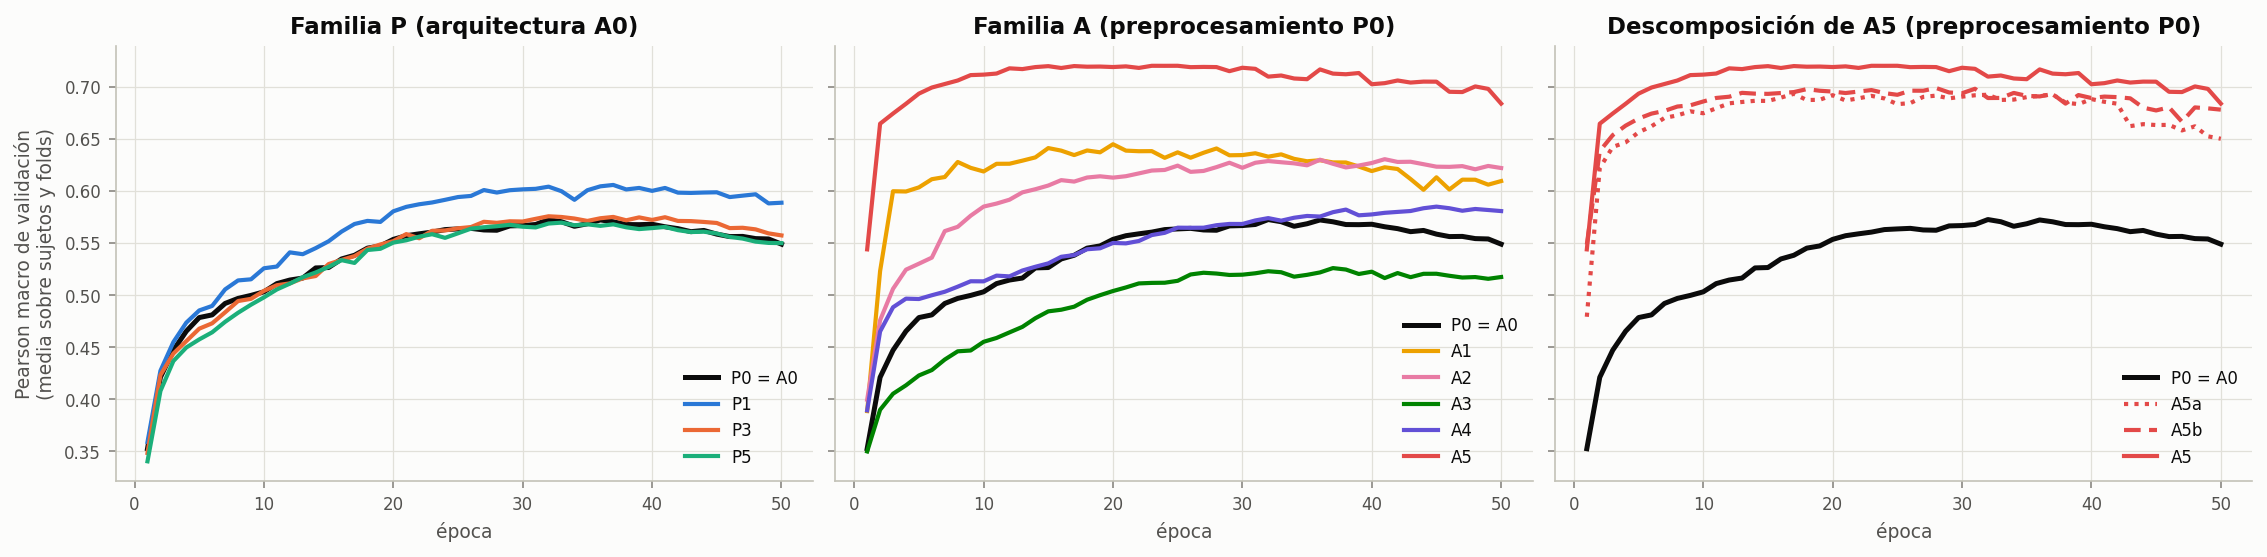
\includegraphics[width=\linewidth,height=0.44\textheight,keepaspectratio]{imgs/training_curves.png}
      \figcap{A.15}{Curvas de validaci\'on de \texttt{A5} donde el \'optimo en \texttt{S1} se alcanza antes de la \'epoca 50. \textbf{Fuente:} Obtenida del repositorio GitHub \cite{rodas_valencia_tpe_ecog}.}
      \vspace{1mm}
      \hfill\hyperlink{anexo:indice_extra}{\beamerbutton{Volver al \'Indice Extra}}
    \end{column}
  \end{columns}
\end{frame}

% --- ANEXO A16: MATEMÁTICA DE TPE, DESCOMPOSICIÓN DE +0.0672 Y VERIFICACIÓN ---
\begin{frame}{Anexo A16: Matem\'atica TPE ($\ell(\lambda)/g(\lambda)$), Descomposici\'on de $+0.0672$ y 60 Folds}{Pregunta del jurado: ?`Cu\'anto mejor\'o realmente TPE durante la b\'usqueda y cu\'anto beneficio persisti\'o al cambiar las semillas?}
  \label{anexo:tpe_diagnostico}
  \begin{columns}[c,onlytextwidth]
    \begin{column}{0.49\textwidth}
      \centering
      \resizebox{\linewidth}{!}{%
        \renewcommand{\arraystretch}{1.16}
        \begin{tabular}{>{\bfseries}l c c c c}
          \toprule
          \rowcolor{ipnDark}
          \textcolor{white}{Transici\'on / Etapa en CV} & \textcolor{white}{\texttt{S1}} & \textcolor{white}{\texttt{S2}} & \textcolor{white}{\texttt{S3}} & \textcolor{white}{Media CV} \\
          \midrule
          1. \texttt{A5} \'epoca 50 fija & $0.6038$ & $0.6216$ & $0.8258$ & $0.6837$ \\
          \rowcolor{rowLight}
          2. \texttt{A5} con checkpoint ($\Delta=+0.0493$) & $0.7103$ & $0.6466$ & $0.8422$ & $0.7330$ \\
          3. Mejor trial TPE ($\Delta=+0.0179$) & $0.7117$ & $0.6879$ & $0.8532$ & $0.7509$ \\
          \rowcolor{rowHighlight}
          4. \texttt{A5} TPE verificado ($\Delta=+0.0041$) & $0.6928$ & $\mathbf{0.6785}$ & $0.8402$ & $\mathbf{0.7372}$ \\
          \texttt{A5b} TPE verificado (60 runs) & $0.6682$ & $0.6540$ & $0.8114$ & $0.7112$ \\
          \bottomrule
        \end{tabular}%
      }
      \fuente{Creaci\'on propia, obtenida del repositorio GitHub \cite{rodas_valencia_tpe_ecog}.}

      \vspace{1.5mm}
      \begin{block}{Diagn\'ostico Estad\'istico del Aporte de TPE}
        \tiny
        \begin{itemize}\setlength{\itemsep}{1.5pt}
          \item \textbf{B\'usqueda ($+0.0179$):} Sujeta al optimismo de elegir el m\'aximo de 32 trials.
          \item \textbf{Verificaci\'on (2 semillas nuevas $\times$ 5 folds):} Ganancia global de $+0.0041$, pero mejora s\'olida y real en \textbf{\texttt{S2} ($\mathbf{+0.0319}$)}. Adem\'as, \texttt{A5} supera a \texttt{A5b} por $\mathbf{+0.0260}$ en los 3 sujetos.
        \end{itemize}
      \end{block}
    \end{column}

    \begin{column}{0.48\textwidth}
      \centering
      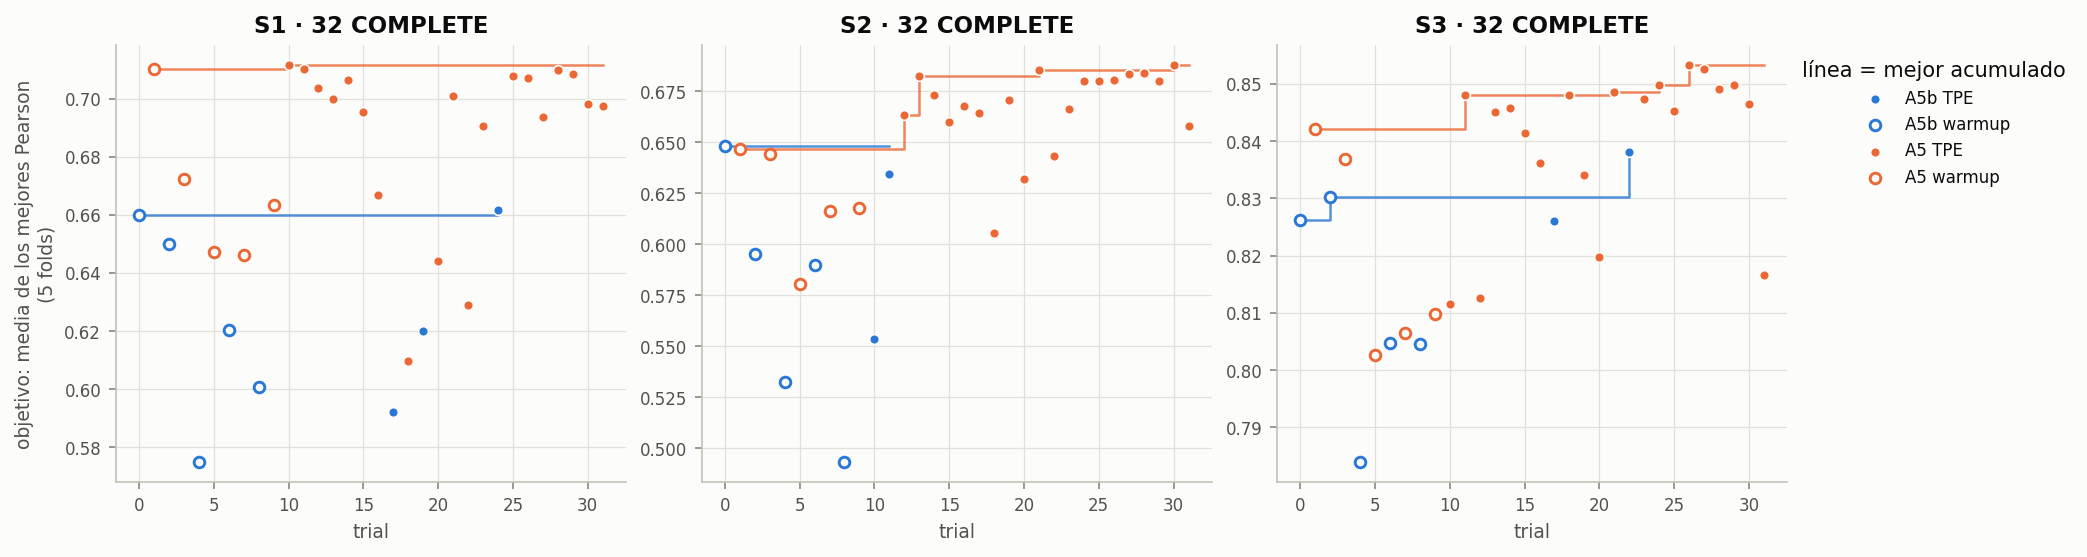
\includegraphics[width=0.48\linewidth,height=0.36\textheight,keepaspectratio]{imgs/optimization_history.png}\hfill
      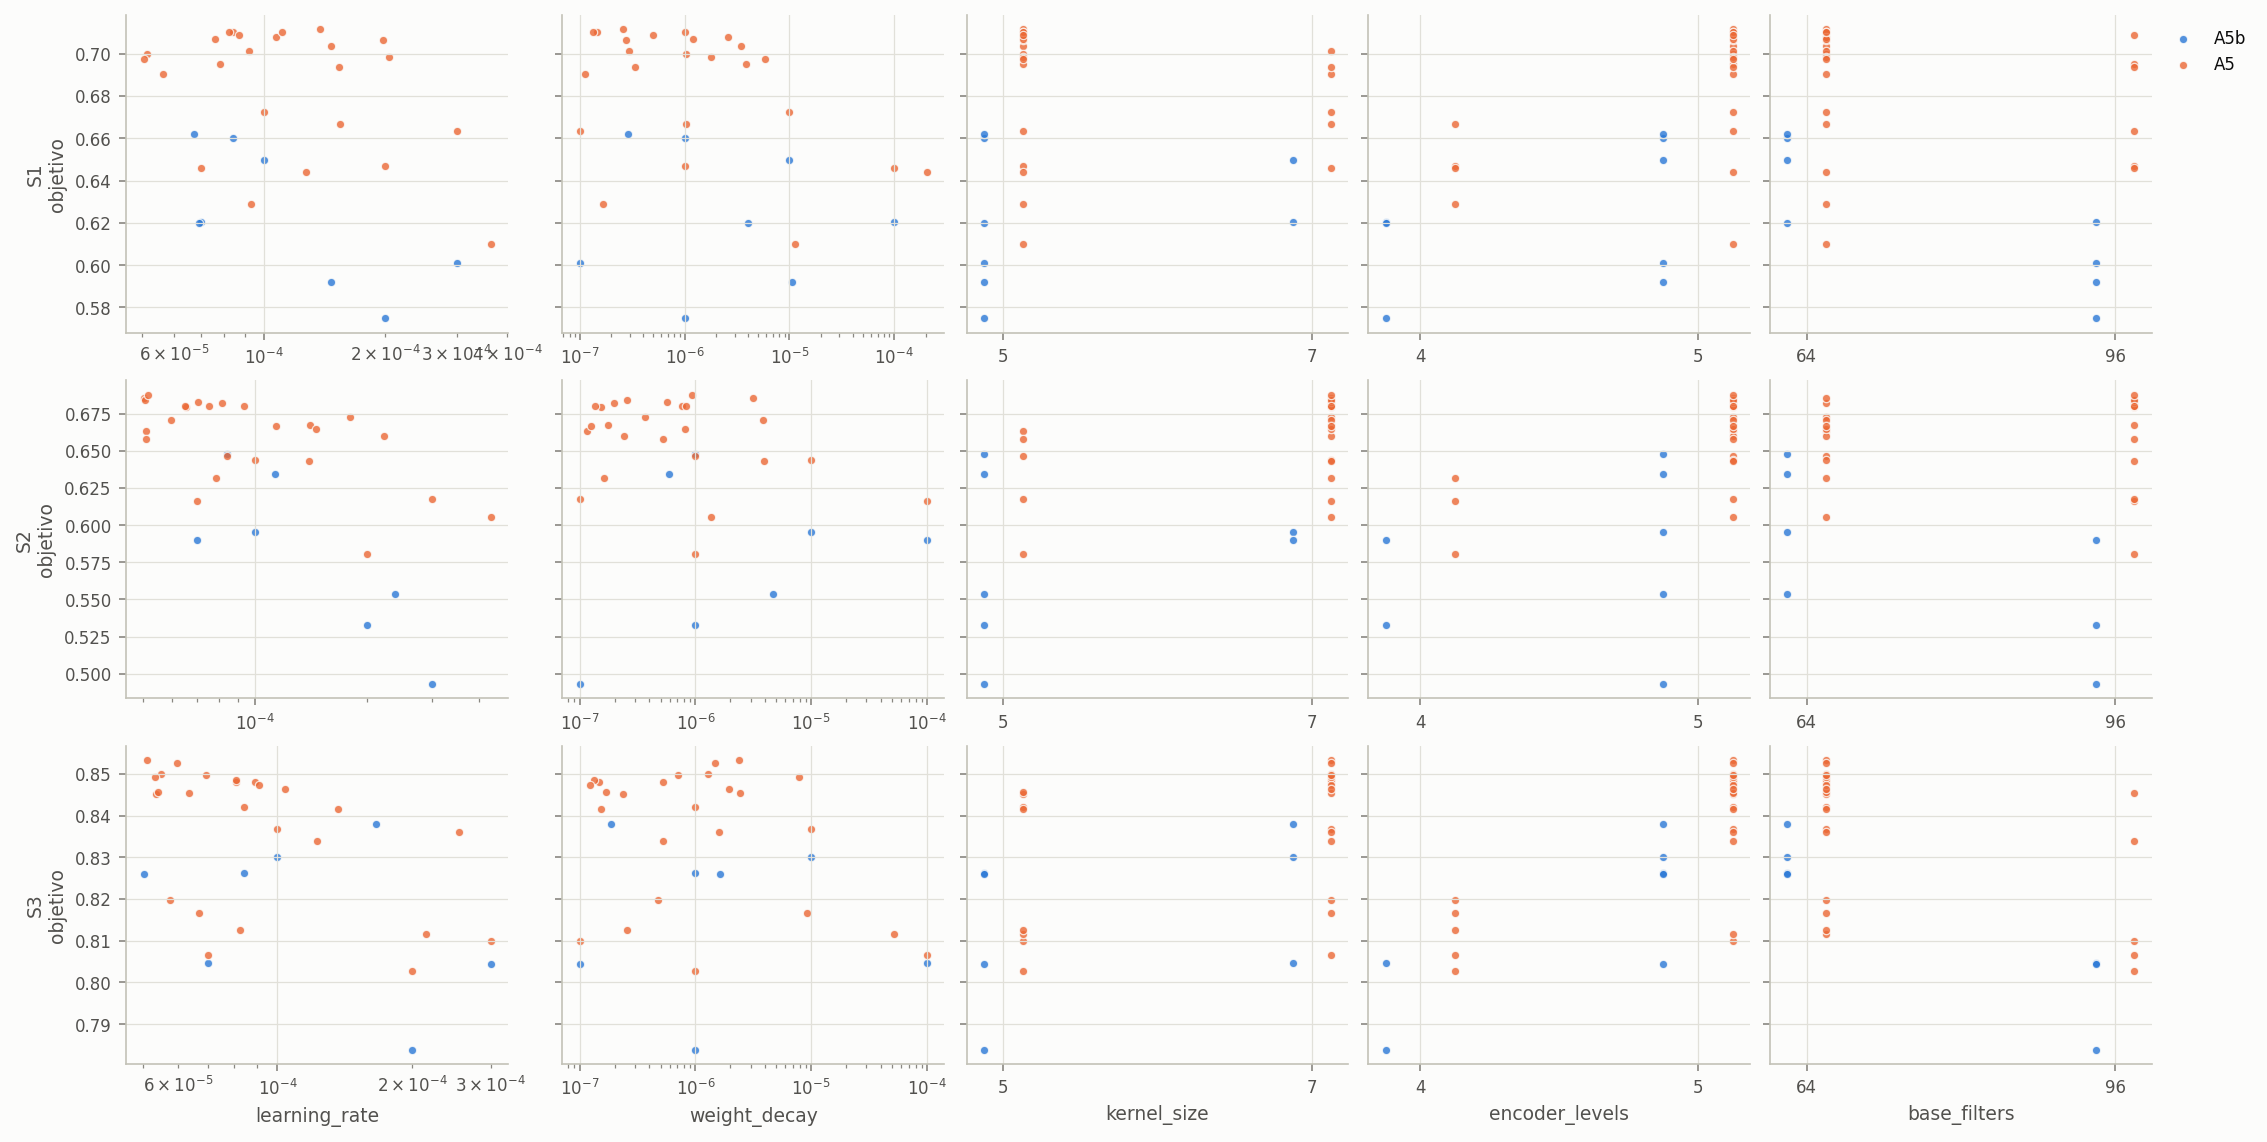
\includegraphics[width=0.48\linewidth,height=0.36\textheight,keepaspectratio]{imgs/params_vs_objective.png}
      \figcap{A.16}{Historial de los 96 trials TPE y relaci\'on par\'ametros vs.\ objetivo. \textbf{Fuente:} Obtenida del repositorio GitHub \cite{rodas_valencia_tpe_ecog}.}
      \vspace{1mm}
      \hfill\hyperlink{anexo:indice_extra}{\beamerbutton{Volver al \'Indice Extra}}
    \end{column}
  \end{columns}
\end{frame}

% --- ANEXO A17: COMPARACIÓN DE PROTOCOLOS DE TEST Y BRECHA CV VS TEST ---
\begin{frame}{Anexo A17: Protocolos de Test ($0.6333$ vs.\ $0.6669$) y Brecha CV vs.\ Test}{Pregunta del jurado: ?`Por qu\'e existe un primer test de $0.6333$ y un segundo de $0.6669$, y por qu\'e difieren del $0.7372$ de CV?}
  \label{anexo:protocolos_test_brecha}
  \centering
  \resizebox{\textwidth}{!}{%
    \renewcommand{\arraystretch}{1.18}
    \begin{tabular}{>{\bfseries}l l c c c c c c}
      \toprule
      \rowcolor{ipnDark}
      \textcolor{white}{Protocolo de Test} & \textcolor{white}{Esquema de entrenamiento final (3 semillas/sujeto)} & \textcolor{white}{\texttt{S1}} & \textcolor{white}{\texttt{S2}} & \textcolor{white}{\texttt{S3}} & \textcolor{white}{Media $r$} & \textcolor{white}{$\operatorname{CCC}$} & \textcolor{white}{$\operatorname{MSE}$} \\
      \midrule
      \texttt{b1b4\_es\_b5} (Inicial) & Entrena en \texttt{B1--B4} + \textit{Early Stopping} monitoreando \texttt{B5} & $0.6087$ & $0.5226$ & $0.7685$ & $0.6333$ & $0.5412$ & $0.6962$ \\
      \rowcolor{rowHighlight}
      \texttt{b1b5\_fixed} (Posterior) & Entrena en \texttt{B1--B5} ($100\%$) + \'epocas fijas ($21, 32, 28$) & $\mathbf{0.6723}$ & $\mathbf{0.5490}$ & $\mathbf{0.7796}$ & $\mathbf{0.6669}$ & $\mathbf{0.5759}$ & $\mathbf{0.6257}$ \\
      \midrule
      \rowcolor{rowLight}
      Diferencia ($\Delta$) & Mejora consistente en $\mathbf{9/9}$ pares sujeto-semilla & $+0.0635$ & $+0.0264$ & $+0.0111$ & $\mathbf{+0.0337}$ & $+0.0347$ & $-0.0705$ \\
      \bottomrule
    \end{tabular}%
  }
  \fuente{Creaci\'on propia, obtenida del repositorio GitHub \cite{rodas_valencia_tpe_ecog}.}

  \vspace{1.5mm}
  \begin{block}{Interpretaci\'on Prudente y Explicaci\'on de la Diferencia entre CV ($0.7372$) y Test ($0.6669$)}
    \scriptsize
    \begin{itemize}\setlength{\itemsep}{2.5pt}
      \item \textbf{Por qu\'e se reportan ambos protocolos (\texttt{tpe\_test\_protocols.csv}):} El salto de $+0.0337$ refleja el cambio de protocolo completo (incorporar \texttt{B5} al entrenamiento y fijar \'epocas de CV); como \texttt{b1b5\_fixed} se formul\'o tras observar $0.6333$, se reporta transparentemente como resultado final exploratorio.
      \item \textbf{Por qu\'e $0.7372$ (CV) vs.\ $0.6669$ (Test) no es una ``ca\'ida de entrenamiento'':} Son mediciones sobre particiones distintas: la CV promedia $5$ bloques internos de desarrollo ($320\text{ s}$), mientras que el Test eval\'ua un segmento temporal futuro e independiente ($200\text{ s}$) sujeto a deriva no estacionaria de la se\~nal ECoG \cite{rodas_valencia_tpe_ecog}. \hfill\hyperlink{anexo:indice_extra}{\beamerbutton{Volver al \'Indice Extra}}
    \end{itemize}
  \end{block}
\end{frame}

% --- ANEXO A18: COMPARACIÓN CELDA A CELDA A5 VS DTCNET ---
\begin{frame}{Anexo A18: Comparaci\'on Celda a Celda por Dedo y Sujeto: \texttt{A5} vs.\ \textit{DTCNet} (2025)}{Pregunta del jurado: ?`C\'omo se comporta nuestro modelo 1D \texttt{A5} frente a \textit{DTCNet} (3D) en cada dedo individual?}
  \label{anexo:comparacion_dtcnet_dedos}
  \begin{columns}[c,onlytextwidth]
    \begin{column}{0.55\textwidth}
      \centering
      \resizebox{\linewidth}{!}{%
        \renewcommand{\arraystretch}{1.16}
        \begin{tabular}{>{\bfseries}l c c c c c c}
          \toprule
          \rowcolor{ipnDark}
          \textcolor{white}{Sujeto (Modelo)} & \textcolor{white}{Pulgar} & \textcolor{white}{\'Indice} & \textcolor{white}{Medio} & \textcolor{white}{Anular} & \textcolor{white}{Me\~nique} & \textcolor{white}{Media} \\
          \midrule
          \texttt{S1} --- \texttt{A5} vs.\ \textit{DTCNet} & $0.6135 / 0.69$ & $\mathbf{0.7909} / 0.76$ & $0.6320 / 0.76$ & $0.7188 / 0.74$ & $\mathbf{0.6061} / 0.60$ & $0.6723 / 0.71$ \\
          \rowcolor{rowLight}
          \texttt{S2} --- \texttt{A5} vs.\ \textit{DTCNet} & $\mathbf{0.6241} / 0.62$ & $0.6087 / 0.67$ & $0.4107 / 0.52$ & $\mathbf{0.6280} / 0.56$ & $0.4733 / 0.58$ & $0.5490 / 0.59$ \\
          \texttt{S3} --- \texttt{A5} vs.\ \textit{DTCNet} & $\mathbf{0.8367} / 0.82$ & $\mathbf{0.7487} / 0.73$ & $0.6798 / 0.72$ & $\mathbf{0.8137} / 0.81$ & $\mathbf{0.8190} / 0.77$ & $\mathbf{0.7796} / 0.77$ \\
          \midrule
          \rowcolor{rowHighlight}
          Media \texttt{A5} vs.\ \textit{DTCNet} & $0.6914 / 0.70$ & $0.7161 / 0.72$ & $0.5742 / 0.67$ & $\mathbf{0.7202 / 0.70}$ & $0.6328 / 0.65$ & $0.6669 / 0.69$ \\
          Diferencia ($\Delta r$) & $-0.0086$ & $-0.0039$ & $\mathbf{-0.0958}$ & $\mathbf{+0.0202}$ & $-0.0172$ & $-0.0231$ \\
          \bottomrule
        \end{tabular}%
      }
      \fuente{Creaci\'on propia a partir de \cite{wang2025dtcnet} y el repositorio GitHub \cite{rodas_valencia_tpe_ecog}.}

      \vspace{1.5mm}
      \begin{block}{Hallazgo Clave de la Comparaci\'on en las 15 Celdas}
        \tiny
        \texttt{A5} \textbf{supera a \textit{DTCNet} \cite{wang2025dtcnet} en 8 de los 15 pares sujeto-dedo}, en la media del \textbf{Sujeto 3 ($0.7796$ vs.\ $0.77$)} y en el promedio global del \textbf{dedo Anular ($+0.0202$)}. M\'as del $\mathbf{83\%}$ de la brecha global proviene exclusivamente del dedo Medio ($-0.0958$).
      \end{block}
    \end{column}

    \begin{column}{0.42\textwidth}
      \centering
      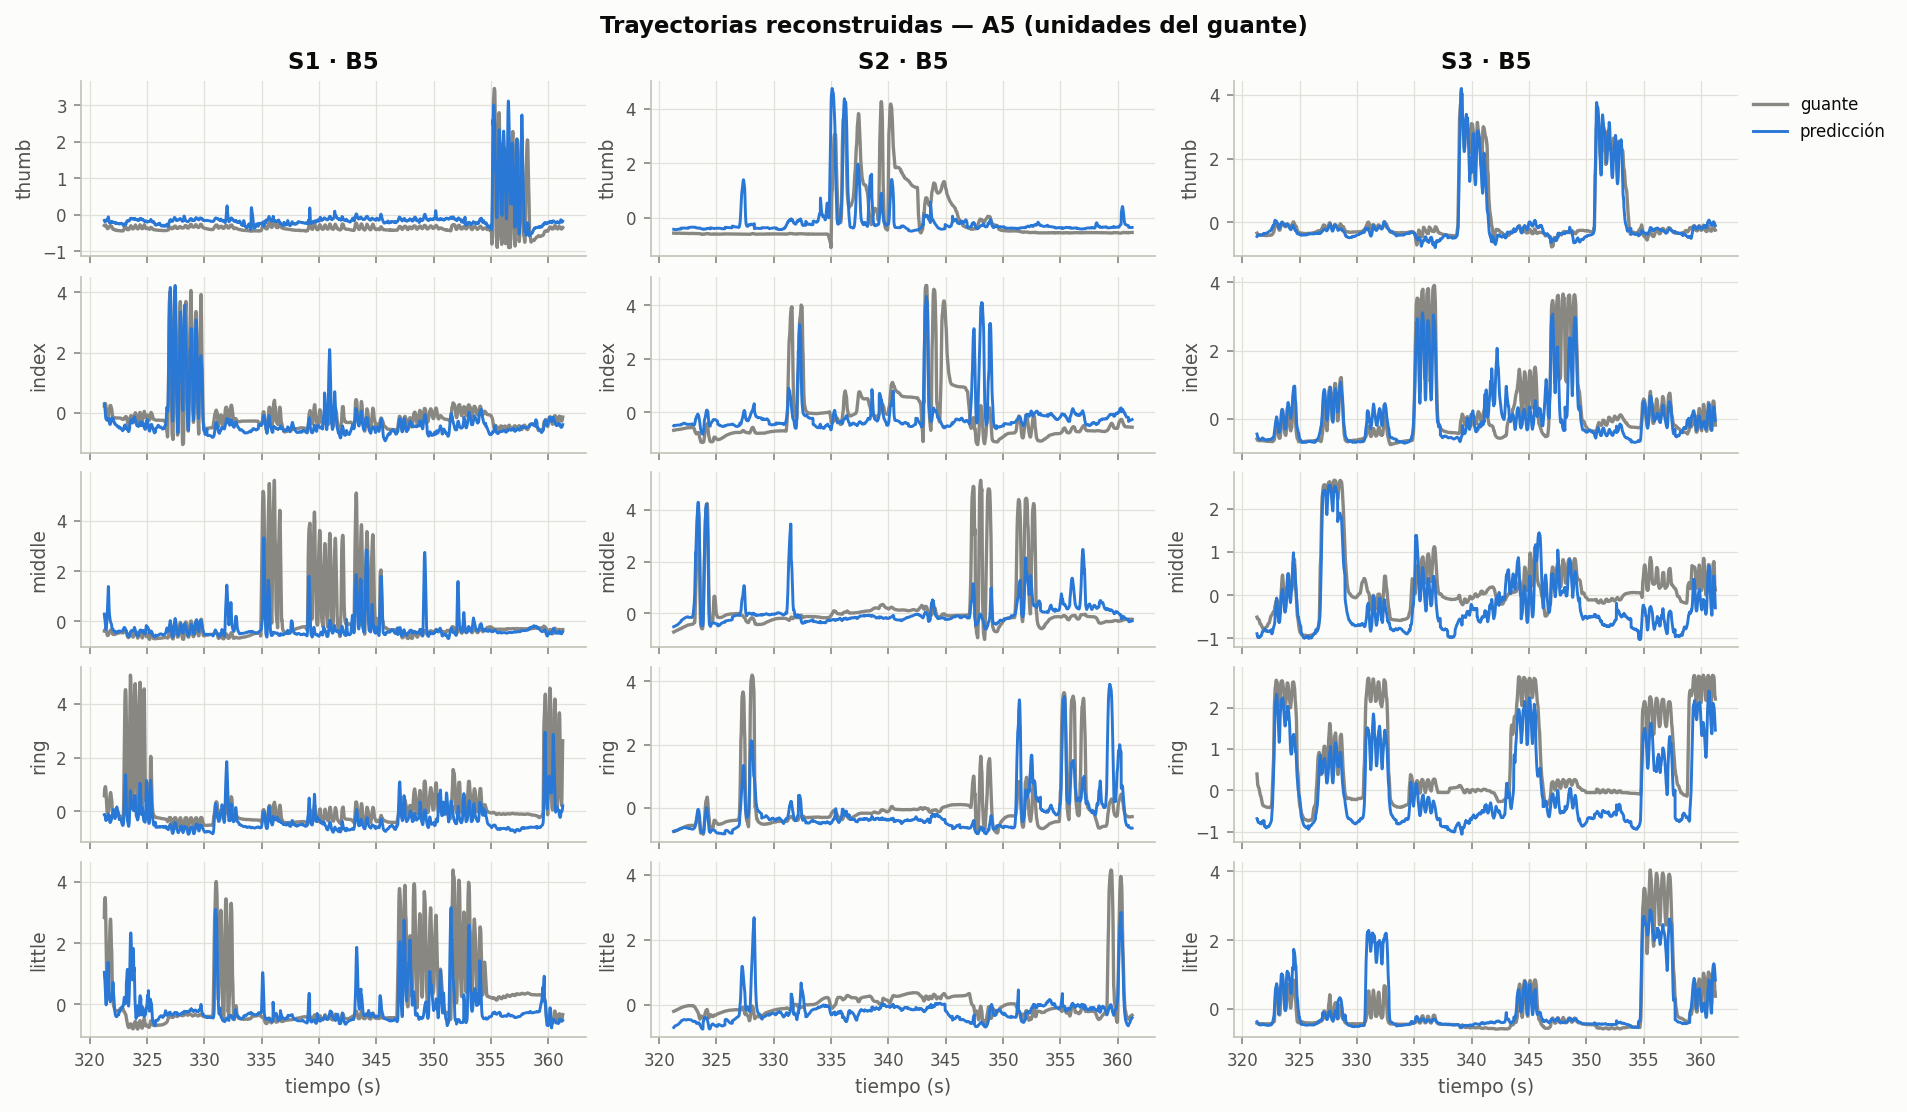
\includegraphics[width=\linewidth,height=0.42\textheight,keepaspectratio]{imgs/example_predictions_A5_B5.png}
      \figcap{A.17}{Reconstrucci\'on de \texttt{A5} en \texttt{B5}. \textbf{Fuente:} Obtenida de GitHub \cite{rodas_valencia_tpe_ecog}.}
      \vspace{1mm}
      \hfill\hyperlink{anexo:indice_extra}{\beamerbutton{Volver al \'Indice Extra}}
    \end{column}
  \end{columns}
\end{frame}

% --- ANEXO A19: MATRIZ DE TRAZABILIDAD COMPUTACIONAL ---
\begin{frame}{Anexo A19: Matriz Completa de Trazabilidad Computacional (Archivos CSV)}{Pregunta del jurado: ?`De qu\'e archivo exacto proviene cada cifra reportada en el documento y en las diapositivas?}
  \label{anexo:trazabilidad_csv}
  \begin{columns}[T,onlytextwidth]
    \begin{column}{0.60\textwidth}
      \centering
      \tiny
      \renewcommand{\arraystretch}{0.95}
      \begin{tabularx}{\linewidth}{>{\ttfamily\color{ipnDark}}l >{\raggedright\arraybackslash}X}
        \toprule
        \rowcolor{ipnDark}
        \textcolor{white}{\normalfont\textbf{Archivo CSV de Respaldo}} & \textcolor{white}{\textbf{Contenido Experimental Auditado (Secci\'on 9)}} \\
        \midrule
        results\_subjects.csv & Medias por sujeto en ablaciones (\'epoca 50, \texttt{A0--A5}, \texttt{P0--P5}). \\
        \rowcolor{rowLight}
        results\_all.csv & Resultados por pliegue, sujeto y dedo en ablaciones. \\
        history\_A5b / history\_A5.csv & Curvas train/val \'epoca por \'epoca ($1\text{--}50$). \\
        \rowcolor{rowLight}
        paired\_deltas[\_summary].csv & Deltas apareados por pliegue ($\texttt{A0}\to\texttt{A5}$, $14/15$ $+$). \\
        summary/ablation\_retrospective.csv & Simulaci\'on retrospectiva de checkpoint ($0.6837 \to 0.7330$). \\
        \rowcolor{rowLight}
        summary/tpe\_trials / tpe\_folds.csv & Historial de los $96$ trials TPE y m\'etricas por fold/par\'ametros. \\
        summary/tpe\_comparison.csv & Descomposici\'on entre \'epoca 50, checkpoint y TPE. \\
        \rowcolor{rowLight}
        summary/tpe\_verification.csv & Verificaci\'on multi-semilla ($60$ runs: \texttt{A5} $0.7372$ vs.\ \texttt{A5b} $0.7112$). \\
        summary/tpe\_selected\_models.csv & Hiperpar\'ametros ganadores y mediana de \'epoca ($21, 32, 28$). \\
        \rowcolor{rowLight}
        summary/tpe\_verification\_paired*.csv & Contrastes apareados en verificaci\'on (\texttt{S2} $+0.0319$). \\
        summary/tpe\_test[\_summary].csv & Test Oficial por semilla, sujeto y dedo ($r=0.6669$). \\
        \rowcolor{rowLight}
        summary/tpe\_test\_protocols.csv & Comparaci\'on \texttt{b1b4\_es\_b5} ($0.6333$) vs.\ \texttt{b1b5\_fixed} ($0.6669$). \\
        \bottomrule
      \end{tabularx}
      \fuente{Creaci\'on propia a partir de los registros del repositorio GitHub \cite{rodas_valencia_tpe_ecog}.}
    \end{column}

    \begin{column}{0.38\textwidth}
      \begin{block}{6 Reglas Oficiales de C\'alculo}
        \tiny
        \begin{enumerate}\setlength{\itemsep}{1pt}
          \item \textbf{Precisi\'on completa:} Toda media se calcula en coma flotante antes de redondear a $4$ decimales.
          \item \textbf{Jerarqu\'ia:} $5\text{ dedos} \to \text{pliegue/semilla} \to \text{sujeto} \to \text{media global}$.
          \item \textbf{Trayectoria completa:} Pearson medido tras \textit{overlap-add}, nunca en ventanas sueltas.
          \item \textbf{Deltas apareados:} $\Delta r$ calculado sin redondear ($\pm 0.0001$).
          \item \textbf{Verificaci\'on limpia:} Excluye la semilla de b\'usqueda.
          \item \textbf{Cero edici\'on manual:} Exportaci\'on directa desde scripts.
        \end{enumerate}
      \end{block}
      \hfill\hyperlink{anexo:indice_extra}{\beamerbutton{Volver al \'Indice Extra}}
    \end{column}
  \end{columns}
\end{frame}

% --- ANEXO A20: GOBERNANZA DE DATOS Y PODA ESTRUCTURADA ---
\begin{frame}{Anexo A20: Gobernanza de Datos Biom\'edicos y Poda Estructurada (Trabajo Futuro)}{Pregunta del jurado: ?`C\'omo se cumple el manejo de datos sensibles y c\'omo reducir el tama\~no ($9.35\text{--}28.03\text{ M}$) para un sistema embebido?}
  \label{anexo:poda_y_privacidad}
  \begin{columns}[T,onlytextwidth]
    \begin{column}{0.45\textwidth}
      \begin{block}{1. Gobernanza y Anonimizaci\'on de Datos Cl\'inicos}
        \scriptsize
        \begin{itemize}\setlength{\itemsep}{3pt}
          \item \textbf{Benchmark p\'ublico internacional:} Se utiliz\'o exclusivamente el corpus \textit{BCI Competition IV --- Dataset 4} \cite{miller2008prediction}, recolectado en el \textit{Harborview Medical Center} (University of Washington).
          \item \textbf{Anonimizaci\'on de origen:} Los registros ECoG se distribuyen desprovistos de metadatos personales (\texttt{sub1}, \texttt{sub2}, \texttt{sub3}), cumpliendo con los protocolos internacionales de privacidad biom\'edica.
        \end{itemize}
      \end{block}
    \end{column}

    \begin{column}{0.52\textwidth}
      \begin{block}{2. Formulaci\'on Proyectiva de Poda Estructurada (Trabajo Futuro)}
        \scriptsize
        Para comprimir las capas profundas ($4f$ y $8f$) de \texttt{A5} hacia hardware neuroprot\'esico de bajo consumo, se plantea como \textbf{propuesta matem\'atica de trabajo futuro} evaluar la importancia de cada filtro $o \in \{1,\dots,C_{\text{out}}\}$ mediante la norma $\ell_1$ y el factor de escala $\gamma_o$ de \texttt{LayerNorm}:
        \[
          \mathcal{I}_{\ell_1}(o) = \sum_{c=1}^{C_{\text{in}}}\sum_{m=1}^{k} |W_{o,c,m}|, \qquad \mathcal{I}_{\text{LN}}(o) = |\gamma_o|\cdot \|\mathbf{W}_{o,:,:}\|_2
        \]
        eliminando f\'isicamente los canales con menor contribuci\'on antes de reentrenar (\textit{fine-tuning}) o destilar hacia un modelo estudiante ligero \cite{rodas_valencia_tpe_ecog}.
      \end{block}
      \vspace{1mm}
      \hfill\hyperlink{anexo:indice_extra}{\beamerbutton{Volver al \'Indice Extra}}
    \end{column}
  \end{columns}
\end{frame}
